\documentclass{IEEEtran}
\usepackage{amsmath}
\usepackage{graphicx}

\begin{document}
    
\title{Hoot Owl Hoot: Lost Game Durations}
\author{Mike Blemberg}
\maketitle

\section{How a Game is Lost}
In Hoot Owl Hoot, a game is lost when the sun token reaches the final sun space.  This occurs when 13 sun cards have been played and the sun token has been moved 13 times.

\section{Position of The 13th Sun Card}
The probability that the 13th sun card exists at a specific position, $k$, in the deck is calculated using the following information.

\begin{enumerate}
    \item There are a total of 14 sun cards distributed throughout the 50 card deck.
    \item 12 sun cards are distributed in the cards before the 13th sun card.
    \item One sun card is positioned somewhere in the deck after the 13th sun card.
\end{enumerate}

The number of possible ways to distribute 14 suns in a 50 card deck is calculated using a binomial coefficient as shown in Equation \ref{eq:total_combinations}.

\begin{equation} \label{eq:total_combinations}
N_{deck\_combination} = \binom{50}{14}
\end{equation}

The number of possible ways to distribute 12 sun cards before the $kth$ position is calculated similarly in Equation \ref{eq:12_suns_combinations}.

\begin{equation} \label{eq:12_suns_combinations}
N_{12\_sun\_combinations} = \binom{k-1}{12}
\end{equation}

And the number of possible locations for the 14th sun card is simply $50-k$.  As a result, the probability that the 13th sun card is located at position $k$ is calculated in Equation \ref{eq:pdf_13th_sun}.

\begin{equation} \label{eq:pdf_13th_sun}
p(k) = \frac{\binom{k-1}{12} \left( 50-k \right)}{\binom{50}{14}}
\end{equation}



The resulting probability distribution function is shown in Figure \ref{fig:13th_sun_pdf}.

\begin{figure}
  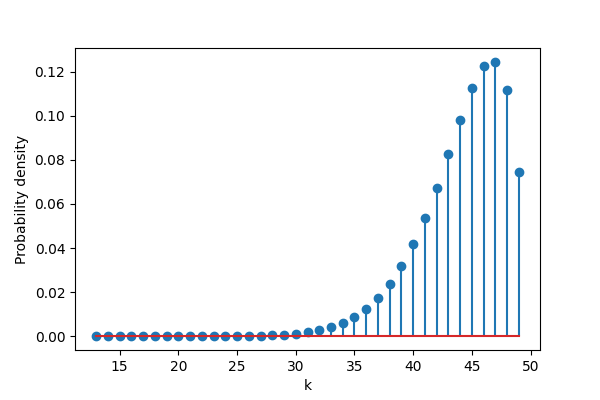
\includegraphics[width=\linewidth]{pdf_13th_sun_position.png}
  \caption{Probability density function for the position, $k$, of the 13th sun card within the deck.}
  \label{fig:13th_sun_pdf}
\end{figure}

The expected position of the 13th sun is calculated in Equation \ref{eq:expected_position_13th_sun}.

\begin{equation} \label{eq:expected_position_13th_sun}
\begin{split}
E[k_{13}] & = \sum_{k=13}^{49}p(k)k \\
& = \sum_{k=13}^{49} \left[ \frac{\binom{k-1}{12} \left( 50-k \right)k}{\binom{50}{14}} \right] \\
& = \sum_{k=13}^{49} \left[ \frac{(k-1)!(50k-k^{2})} {(k-13)!} \frac{14!*36!}{12!*50!} \right] \\
& = 44.2
\end{split}
\end{equation}


\end{document}